\documentclass{article}

\usepackage[utf8x]{inputenc}
\usepackage[frenchb]{babel}
\usepackage[T1]{fontenc}
\usepackage{lmodern}
\usepackage{fullpage}
\usepackage{graphicx}
\graphicspath{{../img/}}
\usepackage{epstopdf}
\usepackage{caption}
\usepackage{subcaption}
\usepackage{multirow}

% Math symbols
\usepackage{amsmath}
\usepackage{amssymb}
\usepackage{amsthm}

% Numbers and units
\usepackage{siunitx}

\DeclareMathOperator{\newdiff}{d} % use \dif instead
\newcommand{\dif}{\newdiff\!}
\newcommand{\fpart}[2]{\frac{\partial #1}{\partial #2}}
\newcommand{\ffpart}[2]{\frac{\partial^2 #1}{\partial #2^2}}
\newcommand{\fdpart}[3]{\frac{\partial^2 #1}{\partial #2\partial #3}}
\newcommand{\fdif}[2]{\frac{\dif #1}{\dif #2}}
\newcommand{\ffdif}[2]{\frac{\dif^2 #1}{\dif #2^2}}
\newcommand{\constant}{\ensuremath{\mathrm{cst}}}

\title{Rapport}
\author{Benoît Legat}

\begin{document}

\maketitle

\section{Resources}
Mettez ici ce que vous trouvez intéressant
\begin{itemize}
  \item Montre comment trouver l'angle et la longueur en comparant Cepstral (mieux pour la longueur et mieux pour l'angle quand la longueur est petite (donc plus pour la caméra que pour le train)) et Radon (mieux pour l'angle avec une grande longueur donc pour le train) et Steerable filters (pourri) \cite{krahmer2006blind}.
  \item Explication de Radon \cite{oliveira2007blind}.
  \item Angle: En gros, il faut voir l'angle des lignes qui sont dans le spectre pour ça il y a: Hough, Radon et Gabor et il conseille Gabor.
    Longueur: Il conseille d'utiliser un Cepstral modifié qu'on utilise et qui marche bien mieux \cite{Deshpande2014606}.
   \item  Rotational Motion Deblurring of a Rigid Object from a Single Image : pour la détection du foreground pour la caméra
   \item  Single Image Motion Deblurring Using Transparency: pour la détection du foreground pour la caméra
\end{itemize}

fft1
rotate in time
black around circle
polar coordinate -> fft2 ou fft1
radon en temporel

\section{Détermination de la PSF}
\begin{figure}[!ht]
  \centering
  \begin{subfigure}[b]{0.45\textwidth}
    \includegraphics[width=\textwidth]{onesFhot.png}
    \caption{Transformée de fourier d'une image unitaire}
    \label{fig:onesFhot}
  \end{subfigure}
  \begin{subfigure}[b]{0.35\textwidth}
    \includegraphics[width=\textwidth]{cameramanFhot.png}
    \caption{Transformée de fourier du caméraman flouté}
    \label{fig:cameramanFhot}
  \end{subfigure}%
  \begin{subfigure}[b]{0.2\textwidth}
    \includegraphics[trim=5cm 0cm 5cm 0cm, clip, width=\textwidth]{cameramanFhotradon.png}
    \caption{Transformée de radon de la transformée de fourier du caméraman non-flouté}
    \label{fig:cameramanFhotradon}
  \end{subfigure}%
  \begin{subfigure}[b]{0.4\textwidth}
    \includegraphics[width=\textwidth]{cameramanvar.png}
    \caption{Variance de la transformée de radon de la transformée de fourier du caméraman flouté}
    \label{fig:cameramanvar}
  \end{subfigure}
  \caption{Tranformées de fourier}
  \label{fig:fourier}
  \begin{subfigure}[b]{0.35\textwidth}
    \includegraphics[width=\textwidth]{cameramanBFhot.png}
    \caption{Transformée de fourier du caméraman flouté}
    \label{fig:cameramanBFhot}
  \end{subfigure}%
  \begin{subfigure}[b]{0.2\textwidth}
    \includegraphics[trim=5cm 0cm 5cm 0cm, clip, width=\textwidth]{cameramanBFhotradon.png}
    \caption{Transformée de radon de la transformée de fourier du caméraman flouté}
    \label{fig:cameramanBFhotradon}
  \end{subfigure}%
  \begin{subfigure}[b]{0.4\textwidth}
    \includegraphics[width=\textwidth]{cameramanBvar.png}
    \caption{Variance de la transformée de radon de la transformée de fourier du caméraman flouté}
    \label{fig:cameramanBvar}
  \end{subfigure}
  \caption{Tranformées de fourier}
  \label{fig:fourier}
\end{figure}

\subsection{Angle estimation}
% TODO, refaire les images en floutant avec circular et en se souvenant de la longueur du flou...
Flouter, c'est faire une convolution en temporelle avec une marche,
ce qui fait une multiplication par $\frac{\sin(x)}{x}$ en fréquentiel.
Cette trace est assez visible.
En effet, sur la transformée de fourier de l'image de départ (figure~\ref{fig:cameramanvar}), il n'y a pas de trace visible alors
que lorsqu'on la floute, on obtient une trace à $\deg{70} + \deg{90}$ (le flou est à $(???, \deg{70})$).
Malheureusement, il y a aussi une croix qui se crée lorsqu'on floute qui est assez présente du fait qu'on a flouté avec ``replicate''.


\subsubsection{Var ou max}
Si on prend le cameraman qu'on tourne à \ang{45}, et qu'on floute à (40, \ang{10}), var donne \ang{3} et max donne \ang{10} !

\subsubsection{Problème de croix}
En \ang{0} et \ang{90}, il y a souvent une marque, indépendemment de l'angle, elles ressemblent même parfois à un $\sin(x)/x$ (voir la voiture de stivy tournée à \ang{45}~\ref{fig:car_cross} ou le cameraman flouté à (40, \ang{10}) tourné de \ang{45}).
C'est à se demandé si ce n'est pas du au fait qu'on prend un rectangle de l'image réel pour fft2
qui est un produit en temporel par deux passe-bas à \ang{0} et \ang{90}
(donc convolution par des $\sin(x)/x$ en fréquentiel ? Ici ça ressemble plus à un produit en fréquentiel...).
Serait-ce une bonne idée de passer en coordonnées polaires avant fft2 et faire fft2 sur l'image en polaire ?

\begin{figure}[!ht]
  \centering
  \includegraphics[width=\textwidth]{car_cross.png}
  \caption{Visible cross}
  \label{fig:car_cross}
\end{figure}

\subsubsection{Solutions}
On va ignorer un interval autour \ang{0} et \ang{90} pour éviter de fausser le calcul.
\paragraph{Première idée}
On prend de \ang{20} à \ang{70} (ainsi que \ang{110} à \ang{160}), puis on tourne l'image de \ang{45} et on refait pareil.
En suit, on prend le max sur tous les vars et si on trouve un de l'image tournée, on fait $-\ang{45}$ à l'angle trouvé.
Pour le cameraman à (40, \ang{10}), on a tout de même \ang{20}.

Le problème c'est que le pic à \ang{10} pour l'image non tournée est bien plus importante que celui à \ang{55} pour l'image trounée.
Du coup, même à \ang{20}, on a encore l'influence du pic.
Il ne faudrait pas se comparer les var ou max de l'original avec celle tournée de \ang{45} ou du moins, pas autant.

Il faudrait prendre le maximum de chaque image indépendemment et puis comparer.
Enfin, pour l'instant ça reste pareil mais si on fait le maximum pour les images séparément, on peut s'assurer qu'on est un pic et pas l'influence d'un pic.

\paragraph{Deuxième idée}
La méthode est la suivante.
\begin{itemize}
  \item Choisir le max de \ang{0} à \ang{179} qu'on nomme $a$.
    Si $a = \ang{0}$ ou $a = \ang{90}$ (éventuellement, plutôt $\max(|a - \ang{0}|, |a-\ang{90}|) < \epsilon$), il faudra trouver un autre $a$ en rognant.
  \item
    Alors tant que $a$ est \ang{0}, \ang{90} ou une valeur au bord d'un rognage (ou à un epsilon près),
    retirer $a$ de la liste des angles (ce qui la rogne).
    On lui rogne donc son début, sa fin (bah oui, si on met un epsilon, il faut aussi prendre 179 en compte ! :P) et son milieu.
\end{itemize}
On fait ça pour chaque orientation de l'image puis on compare la valeur pour les maxs trouvés (c'est ce que j'entends par ``pas autant'' comparer, on compare juste les maxs à la fin).

\section{Quelques résolution avec PSF connue}

\begin{figure}[!ht]
  \centering
  \begin{subfigure}[b]{0.45\textwidth}
    \includegraphics[width=\textwidth]{../matlab/start-nonoise.png}
    \caption{Image de départ}
    \label{fig:start-nonoise}
  \end{subfigure}
  \begin{subfigure}[b]{0.45\textwidth}
    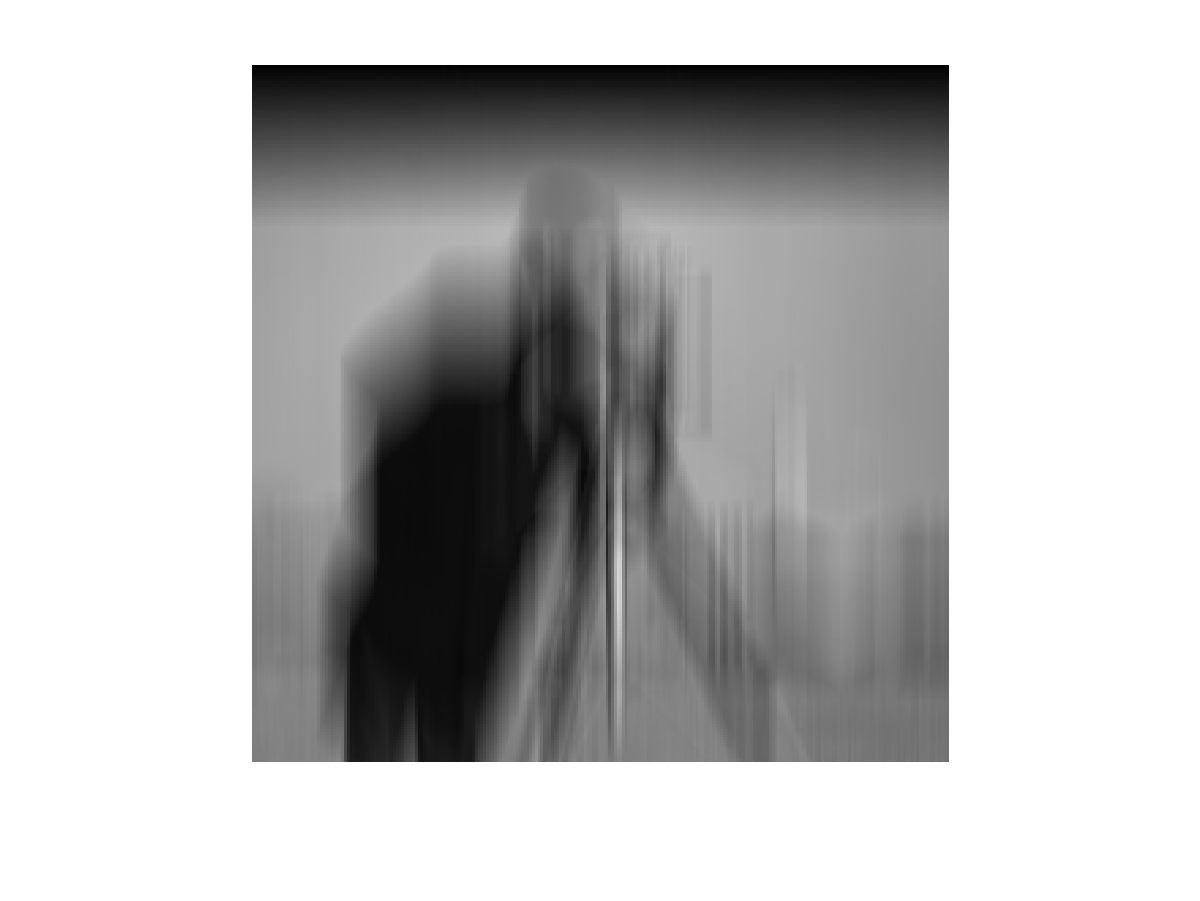
\includegraphics[width=\textwidth]{../matlab/matb-nonoise.png}
    \caption{Image flouté par matrice}
    \label{fig:matb-nonoise}
  \end{subfigure}%
  \begin{subfigure}[b]{0.45\textwidth}
    \includegraphics[width=\textwidth]{../matlab/psfb-nonoise.png}
    \caption{Image floutée par PSF}
    \label{fig:psfb-nonoise_explicite_lambda}
  \end{subfigure}
  \begin{subfigure}[b]{0.45\textwidth}
    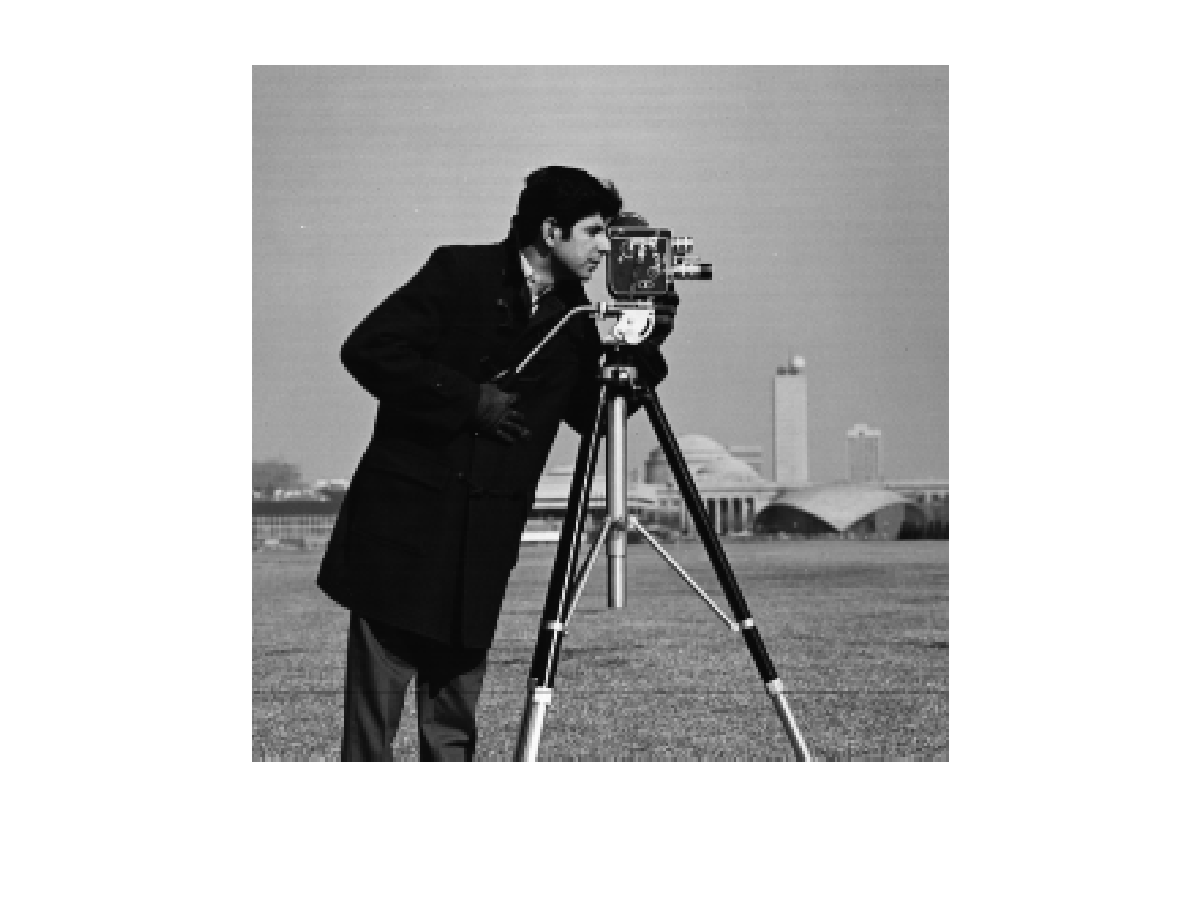
\includegraphics[width=\textwidth]{../matlab/direct-nonoise.png}
    \caption{Image déflouté par méthode directe}
    \label{fig:direct-nonoise}
  \end{subfigure}
  \begin{subfigure}[b]{0.45\textwidth}
    \includegraphics[width=\textwidth]{../matlab/lucy-nonoise.png}
    \caption{Image défloutée par Lucy-Richardson}
    \label{fig:lucy-nonoise}
  \end{subfigure}
  \caption{Résultats pour une image sans noise}
  \label{fig:nonoise}
\end{figure}

\begin{figure}[!ht]
  \centering
  \begin{subfigure}[b]{0.45\textwidth}
    \includegraphics[width=\textwidth]{../matlab/start-noise-g10.png}
    \caption{Image de départ}
    \label{fig:start-noise-g10}
  \end{subfigure}
  \begin{subfigure}[b]{0.45\textwidth}
    \includegraphics[width=\textwidth]{../matlab/matb-noise-g10.png}
    \caption{Image flouté par matrice}
    \label{fig:matb-noise-g10}
  \end{subfigure}%
  \begin{subfigure}[b]{0.45\textwidth}
    \includegraphics[width=\textwidth]{../matlab/psfb-noise-g10.png}
    \caption{Image floutée par PSF}
    \label{fig:psfb-noise-g10_explicite_lambda}
  \end{subfigure}
  \begin{subfigure}[b]{0.45\textwidth}
    \includegraphics[width=\textwidth]{../matlab/direct-noise-g10.png}
    \caption{Image déflouté par méthode directe}
    \label{fig:direct-noise-g10}
  \end{subfigure}
  \begin{subfigure}[b]{0.45\textwidth}
    \includegraphics[width=\textwidth]{../matlab/lucy-noise-g10.png}
    \caption{Image défloutée par Lucy-Richardson}
    \label{fig:lucy-noise-g10}
  \end{subfigure}
  \caption{Résultats pour une image avec noise gaussien}
  \label{fig:noise-g10}
\end{figure}

\begin{figure}[!ht]
  \centering
  \begin{subfigure}[b]{0.45\textwidth}
    \includegraphics[width=\textwidth]{../matlab/start-noise-poisson.png}
    \caption{Image de départ}
    \label{fig:start-noise-poisson}
  \end{subfigure}
  \begin{subfigure}[b]{0.45\textwidth}
    \includegraphics[width=\textwidth]{../matlab/matb-noise-poisson.png}
    \caption{Image flouté par matrice}
    \label{fig:matb-noise-poisson}
  \end{subfigure}%
  \begin{subfigure}[b]{0.45\textwidth}
    \includegraphics[width=\textwidth]{../matlab/psfb-noise-poisson.png}
    \caption{Image floutée par PSF}
    \label{fig:psfb-noise-poisson_explicite_lambda}
  \end{subfigure}
  \begin{subfigure}[b]{0.45\textwidth}
    \includegraphics[width=\textwidth]{../matlab/direct-noise-poisson.png}
    \caption{Image déflouté par méthode directe}
    \label{fig:direct-noise-poisson}
  \end{subfigure}
  \begin{subfigure}[b]{0.45\textwidth}
    \includegraphics[width=\textwidth]{../matlab/lucy-noise-poisson.png}
    \caption{Image défloutée par Lucy-Richardson}
    \label{fig:lucy-noise-poisson}
  \end{subfigure}
  \caption{Résultats pour une image avec noise poisson}
  \label{fig:noise-poisson}
\end{figure}

\bibliographystyle{plain}
\bibliography{biblio}

\end{document}
